\section{Introduction}
\label{sec:intro}

Large language models (LLMs) are increasingly used as natural-language (NL) interfaces for querying tabular data, making Table Question Answering (Table QA) a natural testbed for evidence retrieval, numerical \fg{operations}, and analytical reasoning over structured information. \fg{Most Table QA benchmarks assume that structure is \emph{explicit}, as in clean relational schemas, and that the relevant evidence is contained in a single table or connected through predefined database relations. Many real spreadsheets and reports are instead \emph{non-relational}: the structure needed to answer a question is encoded in the presentation itself, through hierarchical headers, merged cells, blank regions, unit conventions, noisy entries, or implicit dependencies within and across tables}~\cite{1.10}.

This is a blind spot in current Table QA evaluation. A model may answer correctly over a clean relational table yet fail \fg{on a non-relational rendering of the same evidence, especially when that evidence is distributed across multiple tables} (\autoref{fig:nonrelhurts}; \S\ref{app:generating_non_rel}). \fg{Characterizing this failure mode requires controlled benchmarks that preserve the underlying evidence and gold answer across alternative renderings, while allowing systematic variation in domain, layout, perturbations, unit conventions, and cross-table evidence distribution.}
% This is a blind spot in current Table QA evaluation. A model may answer correctly over a clean relational table yet fail when the same latent evidence is rendered as a non-relational view, and this gap widens sharply once the evidence is distributed across multiple tables (\autoref{fig:nonrelhurts}; \S\ref{app:generating_non_rel}). \fg{Systematically studying this gap requires controlled and reliably supervised benchmarks that keep the underlying evidence and gold answer fixed while varying the domain, table layout, perturbations, unit conventions, and distribution of evidence across tables.}
% What is missing is a controlled instrument that keeps the underlying evidence and answer fixed while varying how that evidence is presented, perturbed, and distributed across tables.
% \mlc{la metterei più sul "c'è bisogno di uno strumento che generi questa tipologia di dati on-demand"}
\begin{figure}[t]
    \centering
    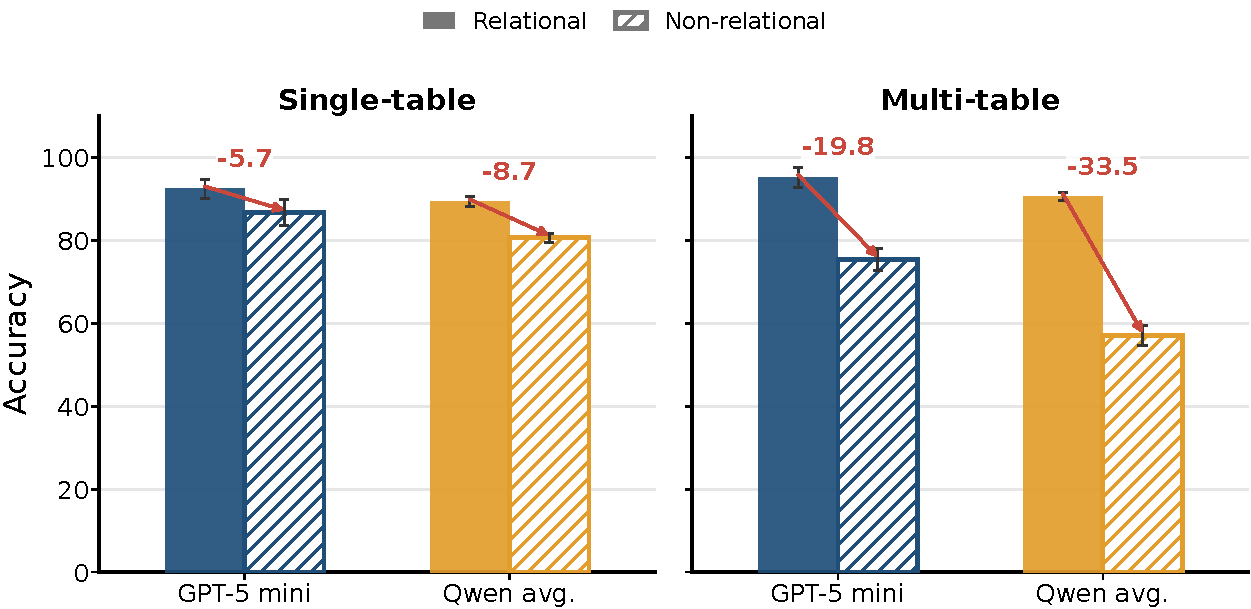
\includegraphics[width=0.48\textwidth]{img/rel_to_nonrel.pdf}
    \caption{Motivating comparison between relational and non-relational presentations: \fg{each question is evaluated on relational and non-relational variants of the same underlying data in both single- and multi-table settings. The figure reports exact-match accuracy (\%) for \texttt{gpt-5-mini} and Qwen-family models on a sample of 192 questions from Spider and Kaggle datasets.}}
    \label{fig:nonrelhurts}
\end{figure}

\begin{figure*}[t]
    \centering
    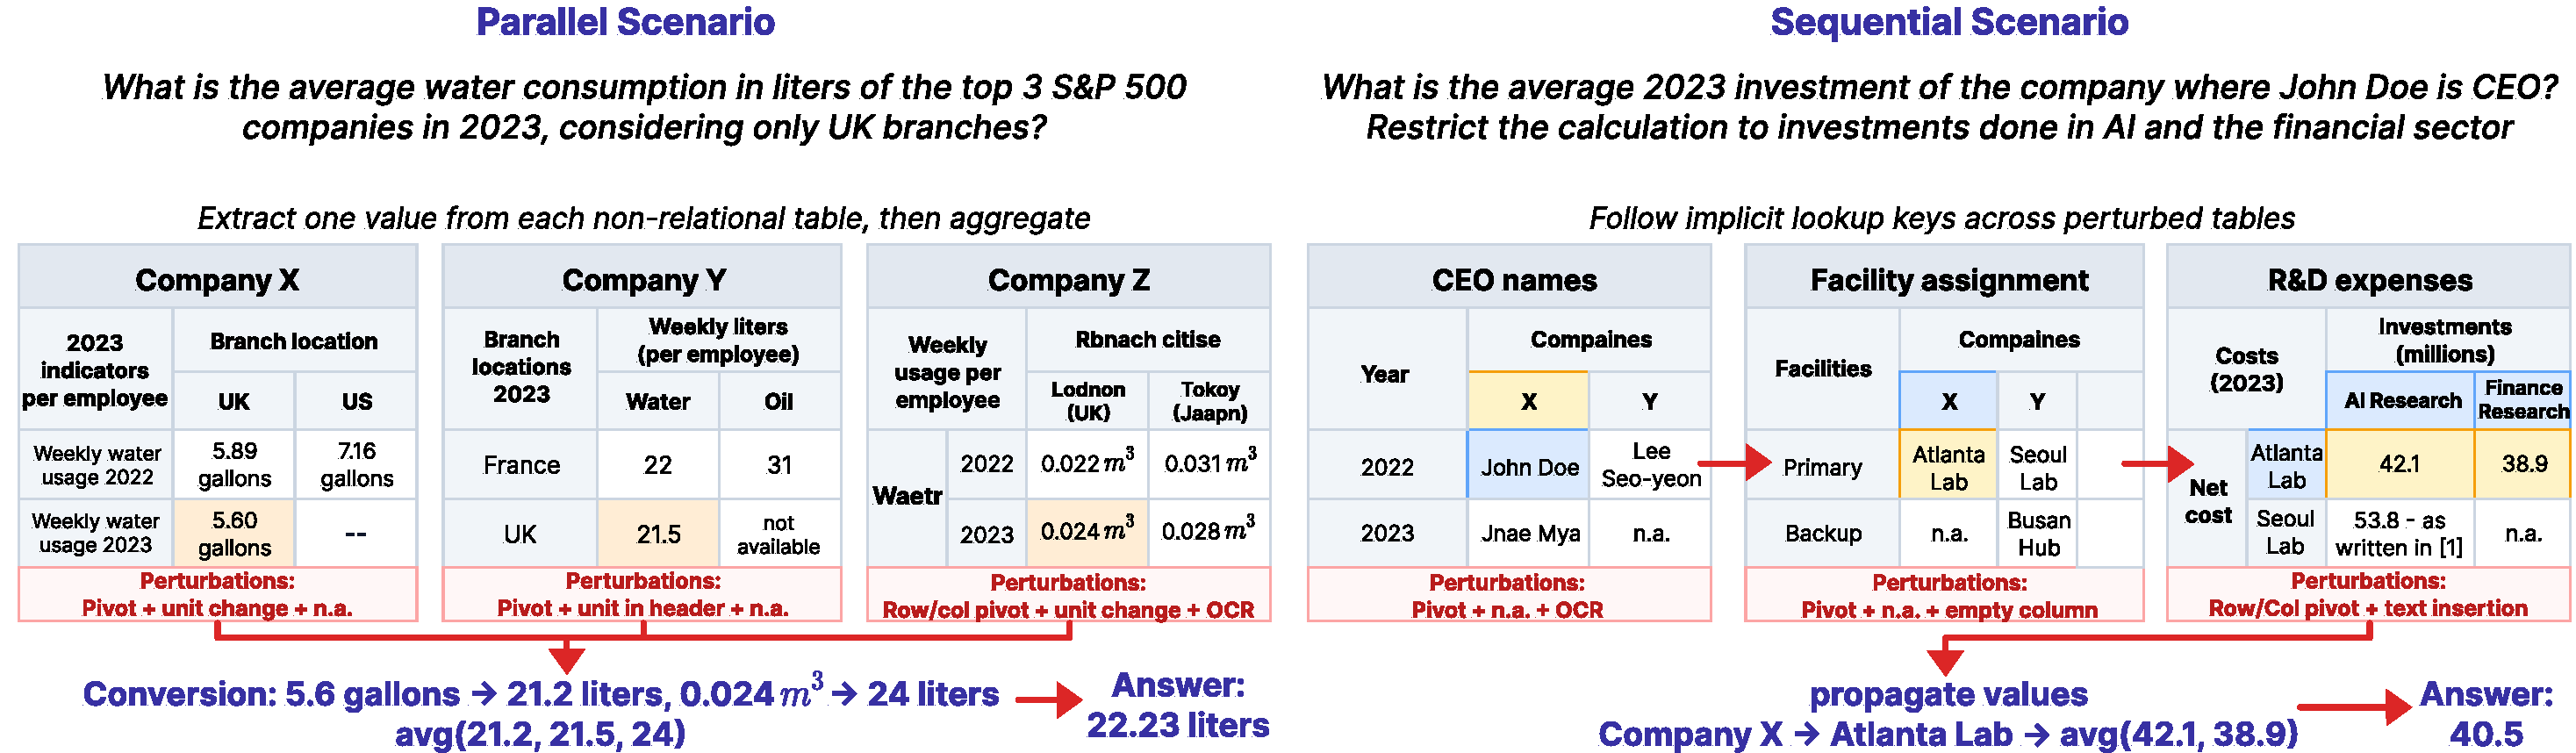
\includegraphics[width=0.99\textwidth]{img/q_types.pdf}
    \caption{\fg{Multi-table parallel and sequential scenarios generated by \name over non-relational tables. Parallel questions extract and aggregate values across perturbed tables; sequential questions propagate lookup keys across tables before aggregating final values.}}
    \label{fig:questiontypes}
\end{figure*}

% Existing resources do not offer this control, for two complementary reasons. manually curated benchmarks span domains such as finance, science, and environmental reporting (\S\ref{sec:rw}), but are fixed in domain and question distribution, rarely target genuinely multi-table reasoning~\cite{1.26,1.16}, and are expensive to build, as realistic tables, questions, perturbations, units, missing values, and gold answers must be designed jointly; this limits scale, domain coverage, and diagnostic control, and raises contamination concerns for recent LLMs~\cite{datacontamination}. 
% Automatic generators are more scalable and verifiable, but remain tied to relational sources: they assume explicit schemas and predefined join paths, and bound the question space to existing database relations~\cite{PapicchioPC23,5.5,5.8}.
% They therefore do not naturally support tables whose structure is conveyed through presentation, nor do they provide direct control over non-relational layouts and implicit dependencies.}

\fg{Current Table QA benchmarks and data-generation methods provide only part of this functionality. Manually curated relational and non-relational benchmarks contain realistic tables (\S\ref{sec:rw}), but they are largely fixed in their domains, layouts, question distributions, reasoning regimes, and number of tables, and only a few target genuine multi-table reasoning settings~\cite{1.26,1.16}. Extending them requires the joint manual design and validation of tables, questions, units, missing values, perturbations, and gold answers. This makes them costly to scale, difficult to adapt to new evaluation scenarios, and potentially exposed to contamination in recent LLMs~\cite{datacontamination}. Automatic data-generation methods provide more scalable and verifiable supervision, but existing approaches are designed around relational databases. They derive questions from explicit schemas, existing relations, and predefined join paths, thereby constraining both the space of generated questions and the ways in which evidence can be selected and distributed across tables~\cite{PapicchioPC23,5.5,5.8}.}

% A natural workaround, i.e., converting relational tables into non-relational ones, is also insufficient, again for two reasons. \emph{Practically}, few real relational tables admit realistic non-relational renderings: as we show in \S\ref{app:generating_non_rel}, only a small fraction of Spider~\cite{1.6}, BIRD~\cite{1.20}, and BEAVER~\cite{1.30} tables can be pivoted into dense or hierarchical layouts without invalid cells, and multi-table constraints are harder still to satisfy. \emph{Conceptually}, multi-table non-relational QA departs from relational joining: in \emph{parallel} settings, models aggregate independent evidence across tables that share neither join keys nor a common schema, whereas in \emph{sequential} settings, they propagate intermediate entities through implicit semantic links rather than explicit keys (\autoref{fig:questiontypes}). A useful benchmark must further vary layouts, surface forms, and unit conventions independently while preserving the gold answer.

\fg{A natural workaround is to convert manually curated or automatically generated relational tables into non-relational views. This approach, however, is insufficient for both practical and experimental-design reasons. Practically, most existing relational tables do not support dense hierarchical renderings: pivoting their attributes often yields sparse layouts or missing combinations. Accordingly, only a small fraction of Spider~\cite{1.6}, BIRD~\cite{1.20}, and BEAVER~\cite{1.30} tables can be transformed into realistic dense or hierarchical views, and the constraints become even stricter when multiple tables must jointly support a question (\S\ref{app:generating_non_rel}). From an experimental-design perspective, post-hoc conversion inherits the schemas, contents, and relationships of the original source, limiting independent control over the reasoning structure, the distribution of evidence, the table presentation, and unit heterogeneity while preserving executable supervision.}

\fg{This lack of control is especially problematic in multi-table QA, which exhibits two complementary evidence-flow patterns (\autoref{fig:questiontypes}): \emph{parallel}, where values independently retrieved from different tables are aggregated, and \emph{sequential}, where intermediate lookup keys are propagated across tables. In non-relational views, the information needed to combine evidence across tables must be recovered from the question and the table contents. Existing approaches do not jointly provide from-scratch table and question generation, executable supervision, non-relational rendering, and controlled variation of both patterns across table count, presentation, perturbations, and unit conventions.}
\fg{}

% \mlc{Non so se abbia senso far partire la lista con "Existing resources do not provide...", inserendo poi anche i punti 3 e 4. Nel senso che si collega bene con i punti 1 e 2 (risorse statiche e generatori dinamici), ma i punti 3 e 4 mi sembrano più dei workaround da applicare a metodi esistenti, che però falliscono nel nostro caso, invece che delle risorse attuali. Forse userei la forma precedente "A natural workaround, i.e. converting ...", ma spiegherei meglio questa distinzione (approcci correnti (1 e 2) vs workaround per far funzionare gli approcci correnti nel caso non-relational (3 e 4))}

% To address these limitations, we introduce \name, a flexible from-scratch framework for generating automatically verifiable QA benchmarks over multiple non-relational tables. Given only a target domain and lightweight generation controls (e.g., attribute cardinalities and table count), \name prompts an LLM to generate a domain-specific schema, instantiates a \emph{latent relational source}, derives executable SQL supervision with scalar answers, and verbalizes the SQL programs into NL questions. Starting from this source, \name renders perturbed \emph{non-relational views}, combining perturbations known to challenge relational QA models~\cite{2.4,2.5,2.6,2.8} %(schema edits, distractors, noisy or missing values)
% with transformations tailored to non-relational tables, such as pivots, hierarchical headers, merged cells, layout restructuring, and unit conversions, and controls how evidence is distributed across views to support \emph{parallel} aggregation and \emph{sequential} propagation.
\fg{We introduce \name, a from-scratch framework for generating automatically verifiable QA benchmarks over multiple non-relational tables, with explicit control over parallel and sequential evidence-flow patterns. Unlike post-hoc conversion, \name synthesizes its own latent source rather than adapting an existing database. Given a target domain and lightweight controls such as attribute cardinalities and table count, \name uses an LLM to define a domain-specific schema and instantiate a \emph{latent relational source}. From this source, it derives executable SQL programs with scalar answers, renders perturbed \emph{non-relational views}, and verbalizes the programs into NL questions. The rendering stage combines established Table QA perturbations~\cite{2.4,2.5,2.6,2.8} with pivots, hierarchical headers, merged cells, layout changes, and unit conversions. This design \emph{decouples supervision from presentation}: answers are computed and verified on the latent relational source, while the model sees only the perturbed non-relational views.}
% the latent relational source computes and verifies answers, while only the perturbed non-relational views are shown to the model. This lets \name vary reasoning topology, perturbations, and answer distributions, and scale the table count to arbitrarily high values, all without changing the gold answers. 
% %\autoref{tab:related_work_comparison} situates \name against prior benchmark- and data-generation approaches: it is the only one to generate tables, questions, and verifiable answers from scratch while applying perturbations under no constraint on the table number.

\begin{table*}[t]
\centering
\fontsize{8.8pt}{10pt}\selectfont
\setlength{\tabcolsep}{1.10pt}
\renewcommand{\arraystretch}{1.15}
\begin{tabular}{llccc cccc}
\toprule
\textbf{Class} &
\textbf{Approach} &
\multicolumn{3}{c}{\textbf{Generated artifacts}} &
\multicolumn{4}{c}{\textbf{Reasoning / evaluation control}} \\
\cmidrule(lr){3-5}
\cmidrule(lr){6-9}
& & Tbl. & NLQ & Ans. & Pert. & Rel. & Non-rel. & \# tables \\
\midrule
\multirow{4}{*}{Perturbation}
& Dr.Spider~\cite{2.6}   & \xmark & \xmark & \xmark & Sch/Txt/Cell & \checkmark & \xmark & SB \\
& EvoSchema~\cite{2.8}   & \xmark & \xmark & \xmark & Sch          & \checkmark & \xmark & SB \\
& ADVETA~\cite{2.5}      & \xmark & \xmark & \xmark & Sch          & \checkmark & \xmark & SB \\
& FREB-TQA~\cite{2.9}    & \xmark & \xmark & \xmark & Cell/Lay     & \xmark     & \checkmark & 1 \\
\midrule
\multirow{3}{*}{\makecell[l]{Tabular\\synthesis}}
& REaLTabFormer~\cite{5.9} & \checkmark & \xmark & \xmark & \xmark & \checkmark & \xmark & N/A \\
& GOGGLE~\cite{5.10}       & \checkmark & \xmark & \xmark & \xmark & \checkmark & \xmark & N/A \\
& TabGen-ICL~\cite{5.1}    & \checkmark & \xmark & \xmark & \xmark & \checkmark & \xmark & N/A \\
\midrule
\multirow{8}{*}{\makecell[l]{QA / SQL\\synthesis}}
& \citet{9.1}           & \xmark     & \xmark     & \checkmark & \xmark & \checkmark & \xmark & 1 \\
& \citet{9.2}           & \xmark     & \checkmark & \checkmark & \xmark & \checkmark & \xmark & 1 \\
& \citet{9.5}           & \xmark     & \xmark     & \checkmark & \xmark & \checkmark & \xmark & SB \\
& ER-Bench~\cite{5.5}   & \xmark     & \checkmark & \checkmark & \xmark & \checkmark & \xmark & SB \\
& SPARTA~\cite{5.8}     & \xmark     & \checkmark & \checkmark & \xmark & \checkmark & \xmark & SB \\
& DSQG-Syn~\cite{9.8}   & \xmark     & \checkmark & \checkmark & \xmark & \checkmark & \xmark & SB \\
& SQLForge~\cite{9.7}   & \checkmark & \checkmark & \checkmark & \xmark & \checkmark & \xmark & SB \\
& SYNQL~\cite{9.6}      & \xmark     & \checkmark & \checkmark & \xmark & \checkmark & \xmark & SB \\
\midrule
\textbf{Ours}
& \textbf{\name}
& \checkmark
& \checkmark
& \checkmark
& \textbf{Sch/Cell/Lay/Num}
& \checkmark
& \checkmark
& \textbf{GC} \\
\bottomrule
\end{tabular}
\caption{
Comparison with data-generation approaches.
Tbl., NLQ, and Ans. denote generated tables, natural-language questions, and automatically verifiable answers.
Perturbations are abbreviated as schema/name (Sch), text/query (Txt), cell/content (Cell), layout/structure (Lay), and numerical/unit (Num).
The number of tables is either fixed to one, source-bounded (SB), or generator-controlled (GC). 
% \fg{\name is the only approach to generate tabular benchmarks from scratch, apply perturbations, and expose generator-controlled table counts.}
}
\label{tab:related_work_comparison}
\end{table*}

\fg{We evaluate \name on financial and environmental scenarios with up to 20 parallel and 5 sequentially connected tables per question, using \texttt{gpt-5-mini} and Qwen-family models. As table count increases, accuracy drops by up to 39.6 points in parallel settings and 32.5 points in sequential settings, while unit heterogeneity causes additional losses of up to 50.1 points, with strong domain dependence. On perturbed real tables, the average accuracy drop caused by non-relational rendering grows from 7.95 points in single-table settings to 30.05 points in multi-table settings. Manual inspection finds 95.9\% of 240 generated questions correct. Finally, \name-generated data improves GRI-QA~\cite{1.16} over the non-finetuned Qwen baseline and complements scarce in-domain supervision, with combined \name and GRI-QA training yielding the best results among the evaluated training regimes.}

In summary, our contributions are:
\fg{(i) we introduce \name, a from-scratch generator of automatically verifiable numerical QA over multiple non-relational tables;}
\fg{(ii) we define controllable parallel and sequential evidence-flow patterns with answer-preserving structural, cell-level, and unit-based perturbations;}
\fg{(iii) we show that table count, non-relational presentation, and unit heterogeneity substantially degrade LLM performance, and confirm on perturbed real tables that non-relationality is especially harmful in multi-table settings;}
\fg{(iv) we validate generated-question correctness and show that \name-generated data provides effective supervision that complements scarce in-domain data;}
\fg{(v) we release code and generated datasets\footnote{\href{https://anonymous.4open.science/r/Gradino-DBF6/}{Anonymous Github link}}.}